\subsection{Performances matérielles}
\subsubsection{Stockage de données}
\par Pour tester les performances de la micro-sd et du disque SDD interne M.2 NVMe, l'utilitaire "hdparm" peut être facilement utilisé. 
{
   \vspace{0.3em} % Adjust the height of the space between caption and tabular
   \renewcommand*{\arraystretch}{1.4}
   \begin{longtable}[t]{@{}|p{25em}|p{2em}|p{2em}|p{3em}|@{}} 
      \caption{Comparaison des performances du "data read" entre un SDD M.2 NVMe et une micro-sd}\label{tab:Timing O_DIRECT disk reads}\\
      \hline
      \textbf{Disk reads} & \textbf{MB} & \textbf{sec} & \textbf{MB/sec}\\
      \hline
      Samsung 970 EVO Plus 250GB M.2 NVMe Internal Solid State Drive & 1004 & 3 & 334.15\\
      \hline
      Microsd card Scan Disk Ultra 32Gb class 10 HC I & 122 & 3.03 & 40.22\\
      \hline
      Microsd card Samsung EVO 64Gb Plus class ? HC 1 & 256 & 3.02 & 84.71\\
      \hline
      Microsd card Samsung EVO 64Gb Select class ? HC 1 & 92 & 3.01 & 30.54\\
      \hline
   \end{longtable}
}
\subsubsection{Performances système}
\par Les diagrammes suivants présentent l'état du nano-ordinateur avant la segmentation, pendant et après. Les indicateurs qui sont observés sont ceux de la mémoire, la fréquence, le I/O, la consommation, la température. Afin de montrer l'impacte potentiel de l'application Chromium, elle est démarrée entre deux segmentations, et pendant la segmentation. 
\par Le test infère en temps réelle la vidéo qui est capturée avec la caméra du nano ordinateur. Le réeseau FCN qui est utilisé est celui fournit par NVIDIA "fcn-resnet18-deepscene-576x320". Ce modèle détecte automatiquement la résolution la plus appropriée avec cette caméra, c'est-à-dire 30 image par seconde (FPS) et une résolution de 1920x1080. Le test dure 1400 secondes, un peu de plus de 23 minutes. Il peut se diviser en onze périodes d'observation, qui sont brièvement décrite ci-dessous: 
\begin{enumerate}
   \item La première période est celle entre la 1re seconde et la 200e seconde, et qui permet d'observer l'état du système au démarrage du nano-ordinateur sans opération mis à part celle de la collecte des statistiques. 
   \item La seconde période est entre la 200e seconde et la 400e, et qui correspond à la première segmentation avec la caméra. Elle permet d'observer le système lors du premier démarrage de la segmentation. 
   \item La troisième période est celle entre la 400e seconde et le premier démarrage de Chromium. Elle permet d'observer la réaction du système après l'arrêt de la segmentation. 
   \item La quatrième période est celle entre le premier démarrage de Chromium et son arrêt. Elle permet d'observer le comportement du système lors de l'utilisation de Chromium, qui est suspecté de ralentir le système, lorsqu'actif (observations faites durant l'essai).
   \item La cinquième période est celle entre l'arrêt de Chromium et le démarrage de la seconde segmentation avec la caméra. Cette période permet d'observer la réaction du système après l'arrêt de Chromium. 
   \item La sixième période est celle entre le démarrage de la seconde segmentation avec la caméra et son arrêt. Cette période permet d'observer la réaction du système pendant la seconde segmentation. 
   \item La septième période est celle entre l'arrêt de la seconde segmentation et le démarrage de la troisième segmentation avec la caméra. Elle permet d'observer la réaction du système après l'arrêt de la segmentation la seconde fois. 
   \item La huitième période est celle entre le démarrage de la troisième segmentation et le démarrage de Chromium la seconde fois. Cette période permet d'observer la réaction du système pendant le démarrage de la segmentation la troisième fois. 
   \item La neuvième période est celle entre le deuxième démarrage de Chromium et son arrêt. Elle permet d'observer le comportement du système lors de l'utilisation de Chromium pendant l'inférence.
   \item La dixième période est celle entre l'arrêt Chromium la seconde fois et l'arrêt de la troisième segmentation. Cette période permet d'observer la réaction du système après l'arrêt de Chromium pendant l'inférence. 
   \item La onzième période est celle entre l'arrêt de la troisième segmentation et l'arrêt du test et de la collecte des statistiques. Elle permet d'observer la réaction du système après l'arrêt de la segmentation la troisième fois. 
\end{enumerate} 
\begin{figure}[H]
   \centering
   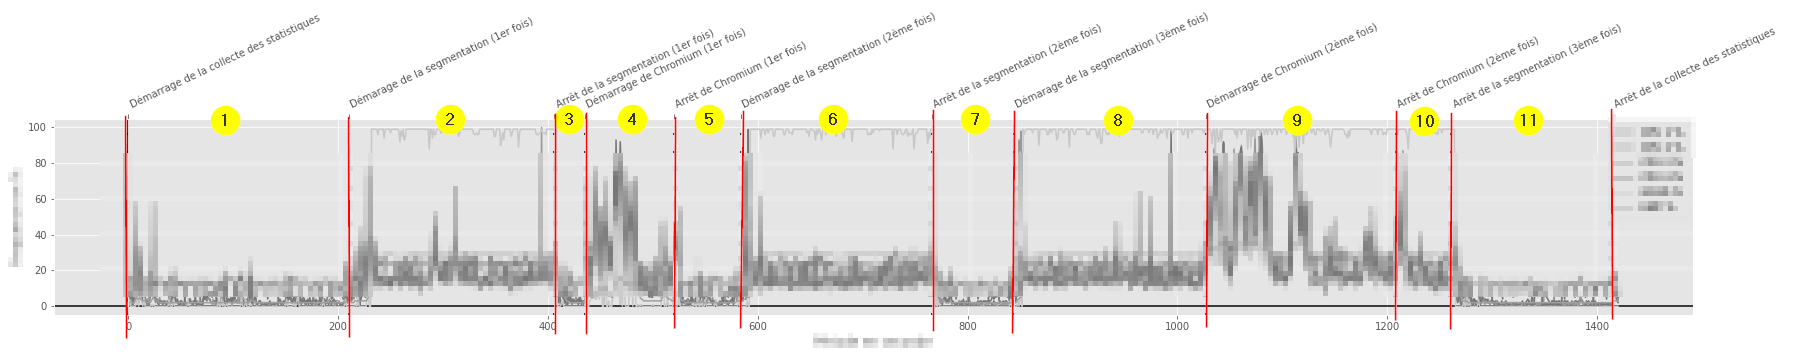
\includegraphics[width=1.0\textwidth]{test_periods}
   \caption{Les périodes du test}
   \label{fig:test_periods}
\end{figure}
{
   \clearpage 
   \newpage
   \begin{landscape}
   \begin{figure}[H]
      \centering
      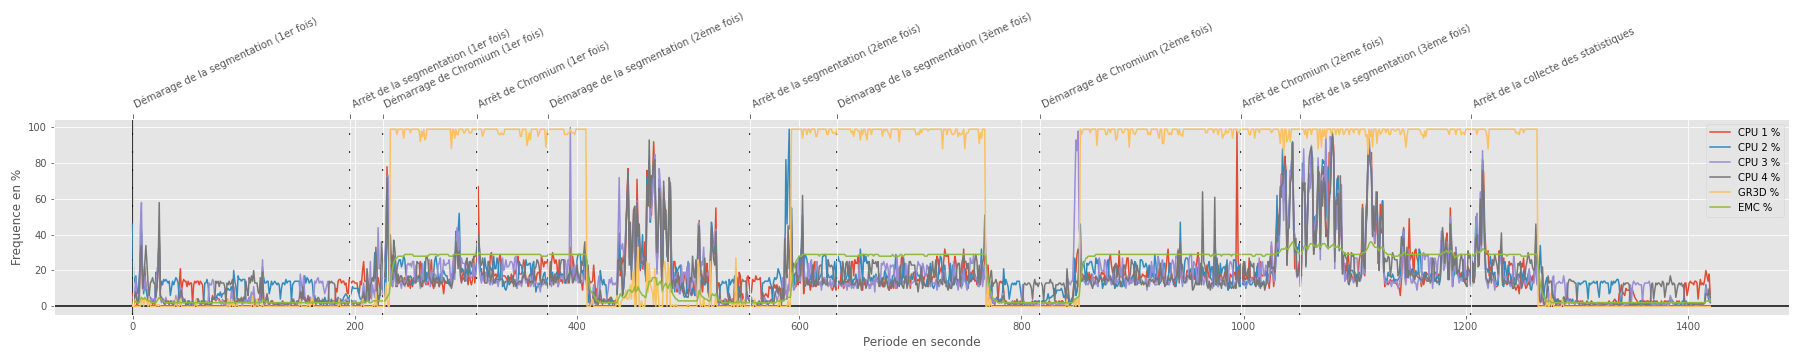
\includegraphics[width=1.5\textwidth]{frequency_usage}
      \caption{Fréquence}
      \label{fig:frequency_usage}
   \end{figure}
   \begin{figure}[H]
      \centering
      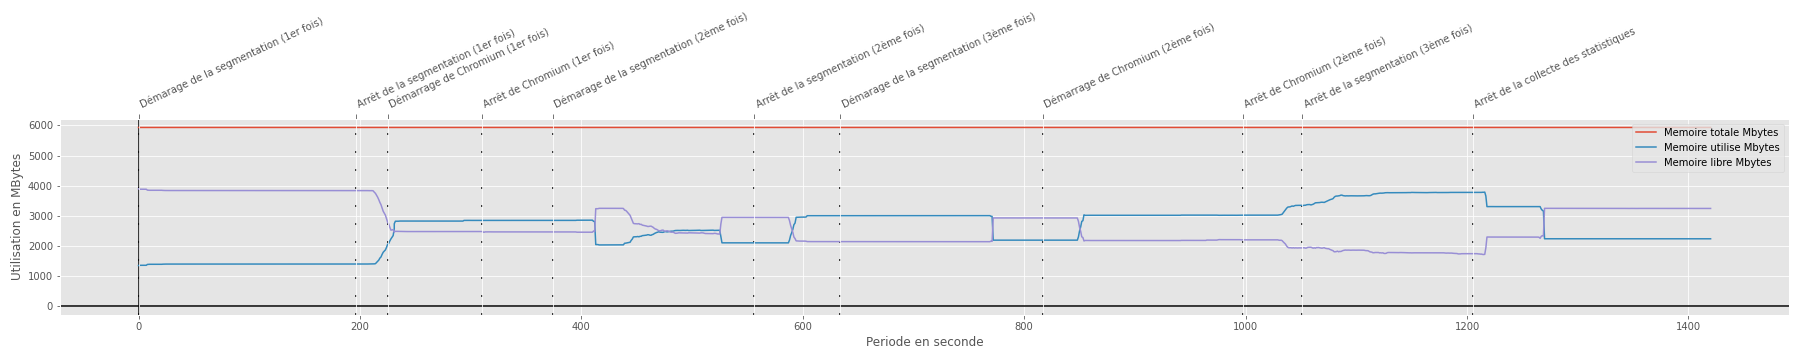
\includegraphics[width=1.5\textwidth]{memory_usage}
      \caption{Mémoire}
      \label{fig:memory_usage}
   \end{figure} 
   \begin{figure}[H]
      \centering
      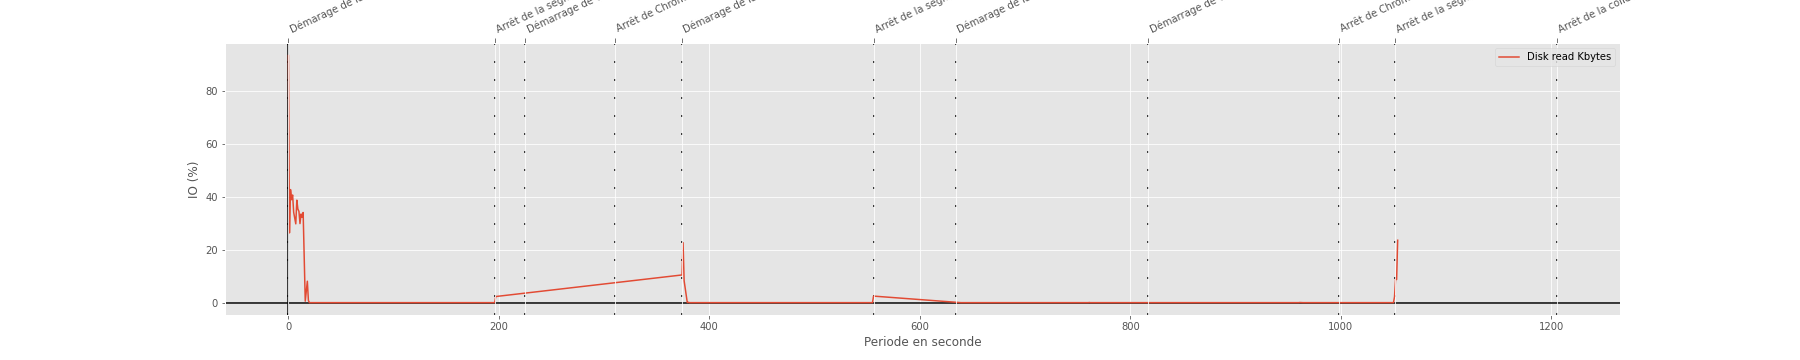
\includegraphics[width=1.5\textwidth]{io}
      \caption{I/O total en \% de la segmentation}
      \label{fig:io}
   \end{figure}
   \begin{figure}[H]
      \centering
      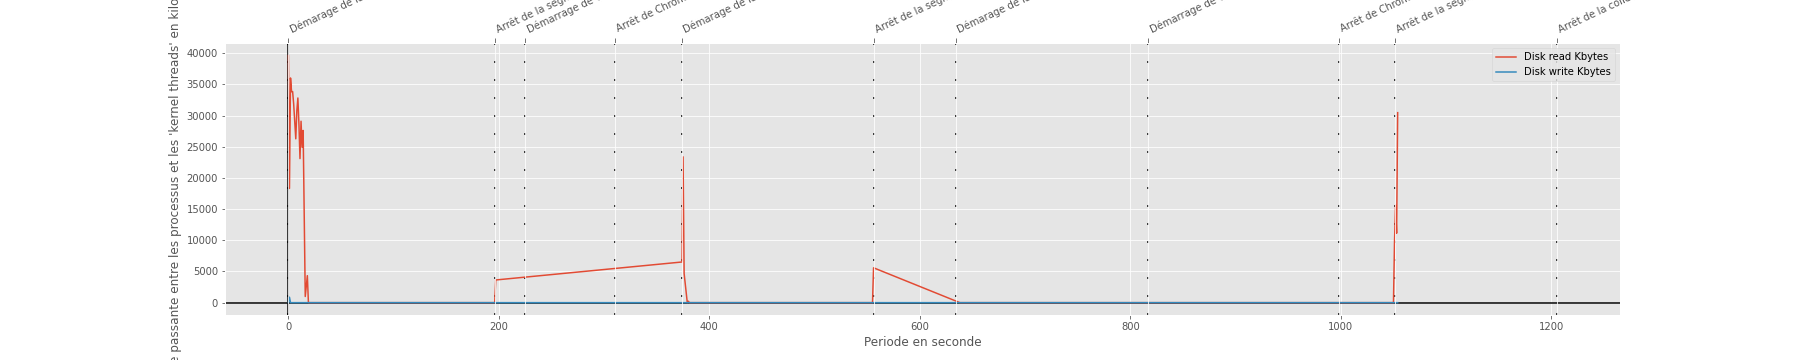
\includegraphics[width=1.5\textwidth]{io_segnetcamera}
      \caption{I/O en KBytes de la segmentation}
      \label{fig:io_segnetcamera}
   \end{figure} 
   \begin{figure}[H]
      \centering
      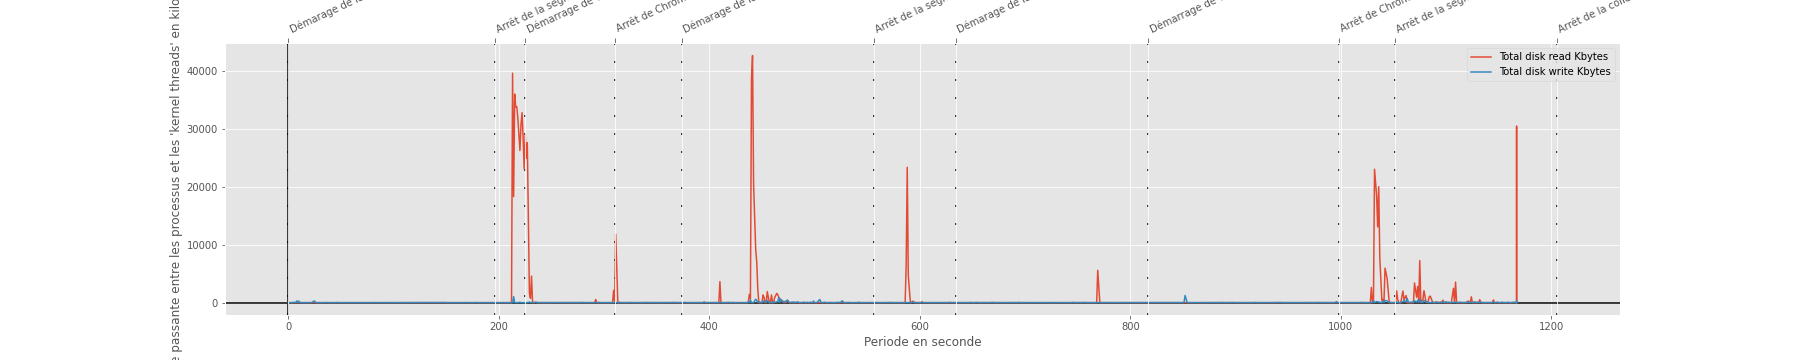
\includegraphics[width=1.5\textwidth]{io_totaldisk}
      \caption{I/O total du disque en KBytes}
      \label{fig:io_totaldisk}
   \end{figure} 
   \begin{figure}[H]
      \centering
      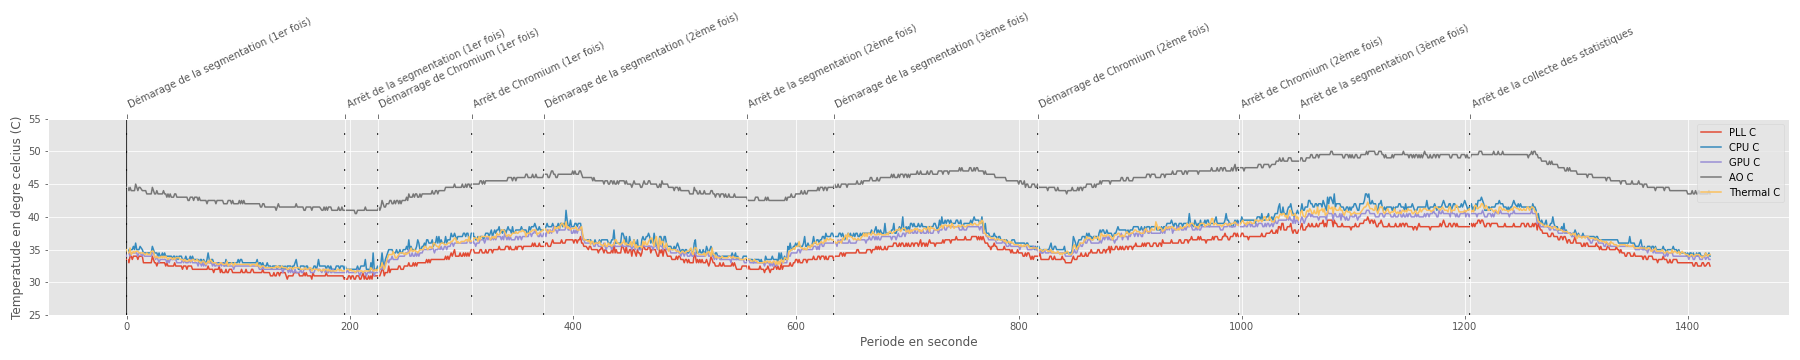
\includegraphics[width=1.5\textwidth]{temperature}
      \caption{}
      \caption[Caption for LOF]{Températures d'opération\protect\footnotemark}
      \label{fig:temperature}
   \end{figure} 
   \footnotetext{PLL: Phase locking loop thermal sensor; AO: Always on thermal sensor. \url{https://forums.developer.nvidia.com/t/operating-temperature-range-on-jetson-nano/73555/10}}
   \begin{figure}[H]
      \centering
      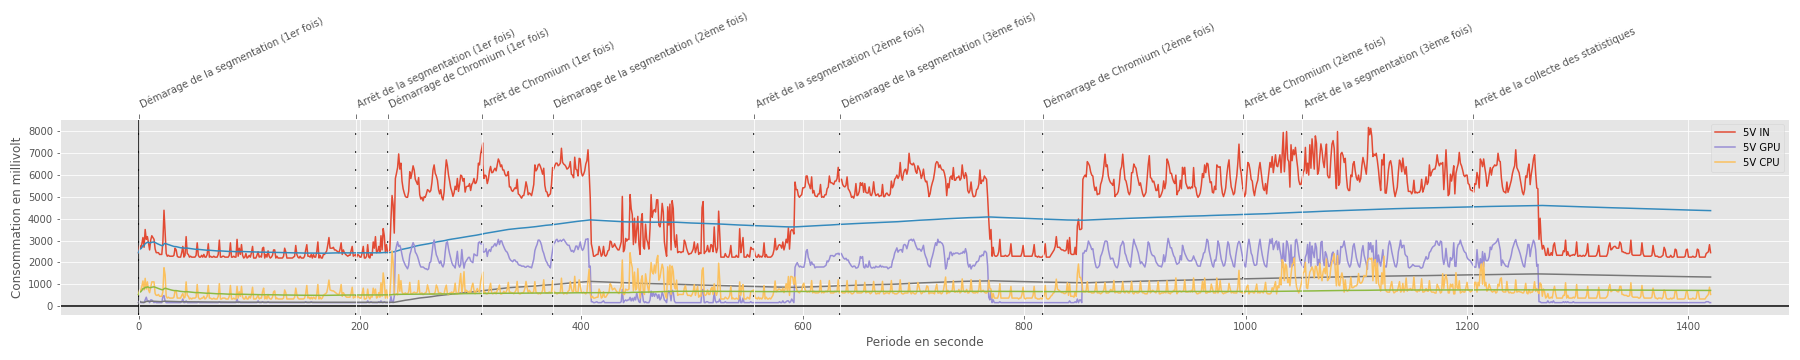
\includegraphics[width=1.5\textwidth]{consommation}
      \caption{Consommation d'opération}
      \label{fig:consommation}
   \end{figure}
   \end{landscape}
   \clearpage
   \newpage
}
\subsection{Performances de l'inférence}
\subsubsection{Images}
\par Les tests ont été fait avec le modèle "fcn-resnet18-deepscene-576x320" fournit par NVIDIA. 
\par Lors de l'entrainement et l'inférence, le script montre un IoU moyen du modèle de 75\%. Mais l'objet d'intérêt de l'essai n'est pas la qualité de la segmentation de l'image complète, mais seulement de la piste cyclable. Certains efforts ont dû être dépensés\footnote{\url{https://github.com/vince7lf/vince7lf.github.io/blob/master/_notebooks/2020-06-21-image_pred_color.ipynb}} afin de pouvoir observer le IoU et le Z-score (Dice) de la segmentation sémantique de la piste cyclable uniquement.
\par Le résultat de la segmentation sémantique peut-être visualisé avec ces deux photos, prises du jeu de donnée de test de la forêt de Freiburg et utiliser comme jeu de données de test pour le modèle. L'image utilisée possède une version vérité terrain ("ground truth")". L'image générée est l'image prédite et peut être comparée avec l'image vérité terrain ("ground truth"), tant que la palette de couleur est identique à la version vérité terrain ("ground truth")". 
\par Il s'avère que le IoU et Dice score sont assez élevés pour les deux photos. 
\begin{figure}[H]
   \centering
   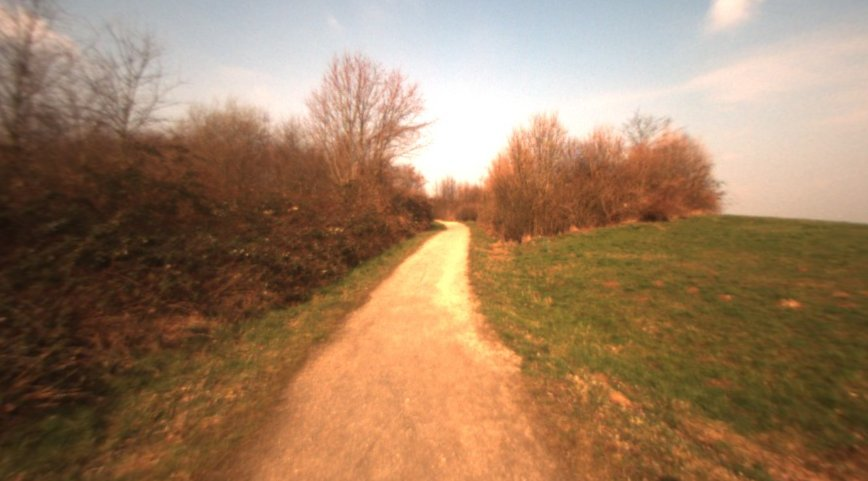
\includegraphics[width=1\textwidth]{b1-09517_Clipped}
   \caption{vérité terrain ("ground truth")" de l'image b1-09517}
   \label{fig:b1-09517_Clipped}
\end{figure}
\begin{figure}[H]
   \centering
   
\includegraphics[width=1\textwidth]{b1-09517_Clipped_pred_new_color}
   \caption{Segmentation sémantique de l'image b1-09517 générée par le modèle. Le IoU et le Dice score pour le chemin sont de +80\%.}
   \label{fig:b1-09517_Clipped_pred_new_color}
\end{figure}
\begin{figure}[H]
   \centering
   
\includegraphics[width=1\textwidth]{b378-61_mask}
   \caption{vérité terrain ("ground truth")" de l'image b378-61}
   \label{fig:b378-61_mask}
\end{figure}
\begin{figure}[H]
   \centering
   
\includegraphics[width=1\textwidth]{b378-61_mask_pred_new_color}
   \caption{Segmentation sémantique de l'image b378-61 générée par le modèle. Le IoU pour le chemin est +69\%.}
   \label{fig:b378-61_mask_pred_new_color}
\end{figure}
\subsubsection{Vidéos}
\par La segmentation sémantique d'une vidéo de la piste cyclable pour différentes résolutions a été filmée avec un téléphone et est disponible dans le projet Vision Météo Teams de l'université de Sherbrooke. On peut y voir les différentes segmentations se succéder, ainsi que les performances du système et les statistiques "tegrastats". 
\par J'ai tenté de capturer le résultat (vidéos/images) de l'inférence directement depuis le nano, mais ce n'est pas une bonne idée, car trop intrusive. Cela ralentit l'inférence. Il y a en fait deux images qui sont produites par le network: overlay et mask, qui sont directement "rendered" dans un XWindow. 
\par J'ai filmé mon écran avec mon cellulaire. Cela produit une vidéo HD 1080p 30FPS. 
\begin{itemize}
   \item Lien\footnote{\url{https://usherbrooke.sharepoint.com/sites/ProjetVisionMto/Documents\%20partages/General/projet\_visionmeteo/videos/gae724\_lefv2603/resultats/20200221\_020044.mp4}} vers une courte vidéo de quelques secondes démontrant l'inférence en temps réel de la segmentation sémantique d'une vidéo de la piste cyclable du pont Jacques-Cartier dans des conditions ensoleillée, mais avec un angle de vue qui change rapidement. Inférence en 30FPS 1920x1080 avec le "network" "fcn-resnet18-deepscene-576x320";
   \item Lien\footnote{\url{https://usherbrooke.sharepoint.com/sites/ProjetVisionMto/Documents\%20partages/General/projet\_visionmeteo/videos/gae724\_lefv2603/resultats/20200412\_232155.mp4}} vers la vidéo longue de +8 minutes démontrant l'inférence en temps réel de la segmentation sémantique d'une vidéo d'une piste cyclable dans des conditions ensoleillée, mais mouillée et avec de la neige. +8min / 800Mb, une seule vidéo qui montre successivement l'inférence de 60 / 30 / 15 / 1 FPS en 720x1280 / 480x640 / 320x480 / 240x320. Le "network" est "fcn-resnet18-deepscene-576x320". Il est limité à 26FPS et 576x320.
\end{itemize}
\par Voici un tableau montrant les différentes résolutions et FPS qui ont été testés avec le modèle:
{
   \color{red}
   \begin{itemize}
      \item Fonctionne: (320,576), (480,640), (720,1280), (768,1024), (768x1152), (800,1152), (832,1024), (864,1024)
      \item Ne fonctionne pas: (832,1120), (832,1152), (768,1280), (800,1280), (864,1152), (900,1152), (900,1280), (960,1600), (1080,1920), (1024,1024)
      \item Frame-per-secondes (FPS): 60/1 30/1 15/1 1/1
   \end{itemize} 
   \todo{TODO}
}